\chapter{HDF5 C++ Interface}
%\section{Example Section}
%\subsection{Example Subsection}
%\subsubsection{Example Subsubsection}
%\paragraph{Example Paragraph}
%\subparagraph{Example Subparagraph}
\section{Overview}
The acronym HDF stands for hierarchical data format meaning this binary format is allowing to structure the internal objects after the users demand. This structure is quite similar to a file system where data is ordered with folders and sub-folders. For more detailed information see the official C \cite{hdf5cdoc} and C++ \cite{hdf5cppdoc} documentation. The reason why also the C documentation is very important is based on the fact that the C++ implementation is mostly a nice wrapper based on the C implementation. For the exact dependence see table \ref{table:corrs}.
\begin{figure}[ht!]
\centering
\begin{tabular}{|l|l|}
\hline
HDF5 C APIs&C++ Classes\\
\hline
Attribute Interface (H5A)&Attribute\\
Datasets Interface (H5D)&DataSet\\
Error Interface (H5E)&Exception\\
File Interface (H5F)&H5File\\
Group Interface(H5G)&Group\\
Identifier Interface (H5I)&IdComponent\\
Property List Interface (H5P)&PropList and subclasses\\
Dataspace Interface (H5S)&DataSpace\\
Datatype Interface (H5T)&DataType and subclasses\\
\hline
\end{tabular}
\caption{Table of correspondence between C and C++}
\label{table:corrs}
\end{figure}
To use the C++ language features to its most capabilities inheritance is used. This allows reuse of functions, objects and properties over many hierarchy layers. This enforces a strict dependence when sharing or creating objects. To have an overview on the hierarchy look at figure \ref{graph:hierarchy}.

\begin{figure}[ht!]
\centering
\resizebox{\textwidth}{!}{
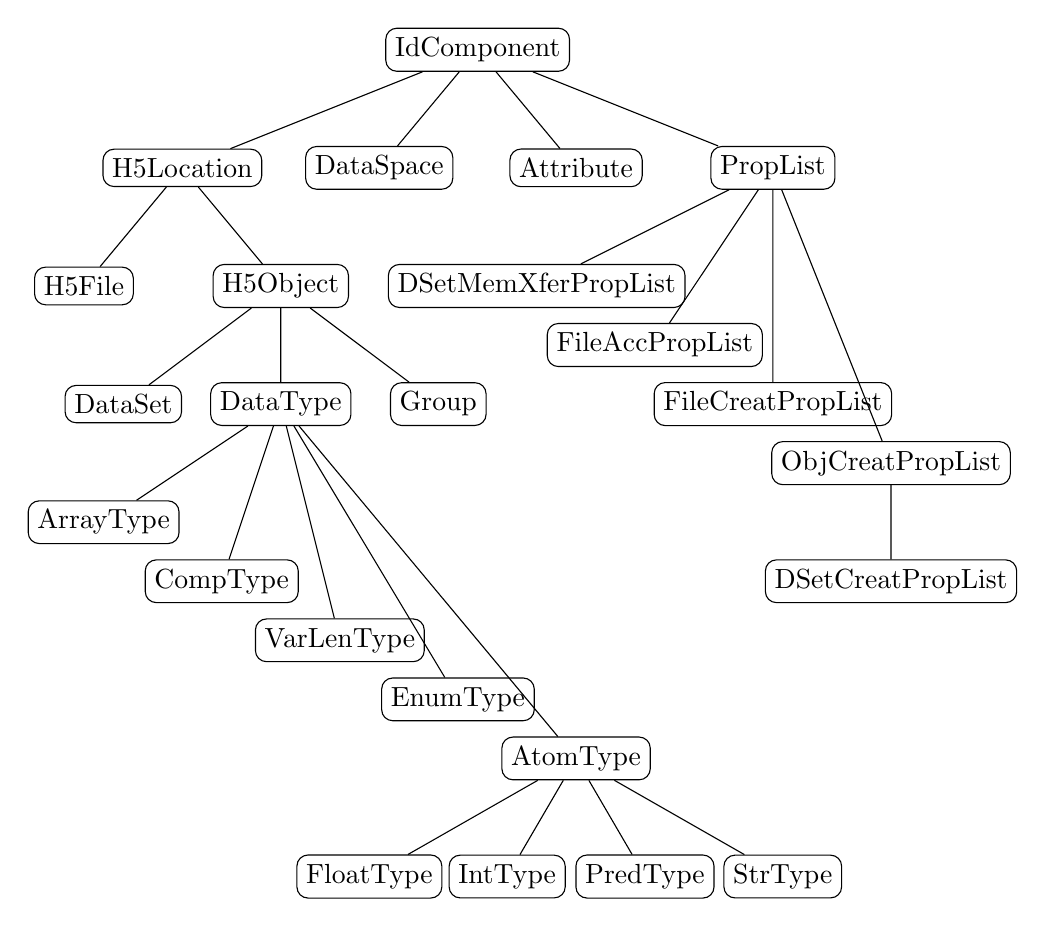
\begin{tikzpicture}[
baseline,
every node/.style = {shape=rectangle, rounded corners, draw, align=center},
]]
  \node {IdComponent}
    child[xshift=-1.5cm]
    {
        node{H5Location}
    	child[xshift=-0.5cm]{node{H5File}}
    	child[xshift=0.5cm]
    		{
    		node{H5Object}
    		child[xshift=-0.5cm]{node{DataSet}}
    		child{
    			node{DataType}
    			child[xshift=0.75cm]{node{ArrayType}}
    			child[xshift=0.75cm,yshift=-0.75cm]{node{CompType}}
    			child[xshift=0.75cm,yshift=-1.5cm]{node{VarLenType}}
    			child[xshift=0.75cm,yshift=-2.25cm]{node{EnumType}}
    			child[xshift=0.75cm,yshift=-3.0cm]
    				{
    				node{AtomType}
    				child[xshift=-0.375cm]{node{FloatType}}
    				child[xshift=-0.125cm]{node{IntType}}
    				child[xshift=0.125cm]{node{PredType}}
    				child[xshift=0.375cm]{node{StrType}} 
    				}
    			}
    		child[xshift=0.5cm]{node{Group}}
    		}
 	}
    child[xshift=-0.5cm]{node{DataSpace}}
    child[xshift=0.5cm]{node{Attribute}}
    child[xshift=1.5cm]{
    	node{PropList}
    	child[xshift=-0.75cm]{node{DSetMemXferPropList}}
    	child[xshift=-0.75cm,yshift=-0.75cm]{node{FileAccPropList}}
    	child[xshift=-0.75cm,yshift=-1.5cm]{node{FileCreatPropList}}
    	child[xshift=-0.75cm,yshift=-2.25cm]{
    		node{ObjCreatPropList}
    		child{node{DSetCreatPropList}}
    		}
    		};
\end{tikzpicture}
}
\caption{Depiction of derivation hierarchy}
\label{graph:hierarchy}
\end{figure}

As stated in the background this project is about the simulation of \textit{Hagedorn} wavepackets over a fixed time horizon. To keep track and possibly reproduce the results the wavepackets have to be saved in every time step $\Delta t$ of the simulation. This has to be achieved with the classes shown in figure \ref{graph:hierarchy}. To understand the functionality of these classes they will be explained in the following sections.

\section{Internal types and states}
\label{seq:internaltypes}
An interface in general has supported objects and functions. These functions also have preconditions and postconditions whereas objects have valid states. In case of the HDF5 library when these are not fulfilled an exception is thrown which could abort or interrupt the program execution. Therefore it is important to always use valid objects and function calls. There are two noteworthy types which are also used the most. These are \texttt{hsize\_t} and \texttt{H5std\_string}. Variable of type \texttt{hsize\_t} represent native multiple-precision integer. This type substitutes the C++ internal \texttt{int} data type. The \texttt{H5std\_string} type is just an alias for the \texttt{std::string} data type from the standard library. Internal valid states are represented in only uppercase letters and with the C prefix as in table \ref{table:corrs}. For example a valid property list state is \texttt{H5P\_DEFAULT}.

\section{H5File}
\label{seq:h5file}
As the name already suggest this class is used to manage the binary file object. When a \textit{H5File} is default constructed it also allocates a default \textit{Group} root named "/". To construct a \textit{H5File} a minimal number of two arguments is needed. The two additional optional arguments are a \textit{FileCreatPropList} and a \textit{FileAccPropList} which would allow further specification. These would be creation and access properties as suggested by the names. In case of this project they are not needed and the \texttt{H5P\_DEFAULT} is sufficient. For the first mandatory argument, which is the filename, a \texttt{H5std\_string} or as discussed before a string required. The second mandatory argument defines the type of creation which at default has two valid values. These possible values are \textit{H5F\_ACC\_TRUNC} and \textit{H5F\_ACC\_EXCL} which are mutually exclusive. The former truncates the file meaning if it already exists erase all data previously stored in the file. The latter fails if the file already exists under the specified name which ends in an exception. It is advised to work with \textit{H5F\_ACC\_TRUNC} because it is simpler and thus errors will less frequently occur.

\section{Group}
\label{seq:group}
As previously mentioned it is a hierarchical data format. The hierarchy gets implement through the usage of \textit{Groups}. In case of a \textit{Hagedorn} wavepackets and its corresponding energies the structure in figure \ref{graph:file} is preferred as it corresponds to the structure of the python generated data.

\begin{figure}[ht!]
\centering
\resizebox{\textwidth}{!}{
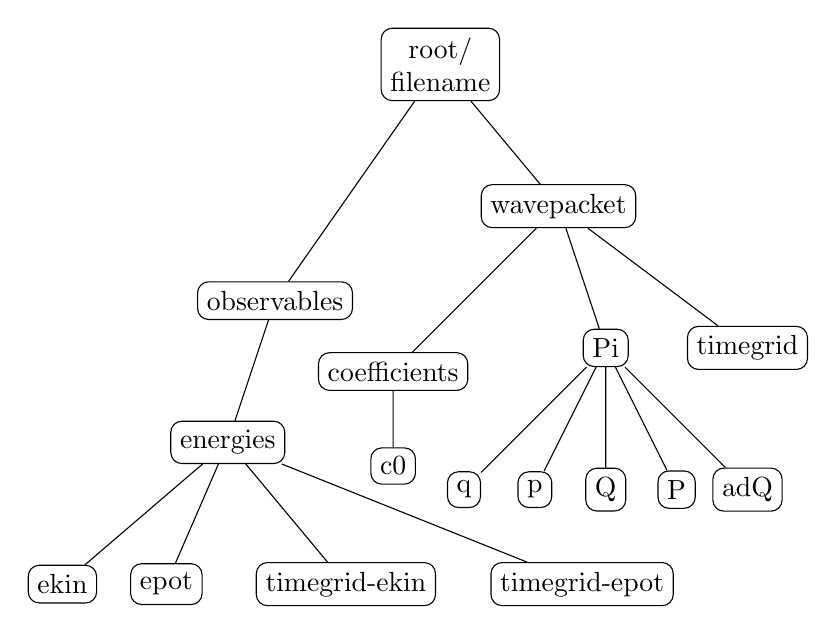
\begin{tikzpicture}[
baseline,
scale=1.2,
every node/.style = {shape=rectangle, rounded corners, draw, align=center},
]]
  \node {root/\\filename}
    child[yshift=-1cm,xshift=-1cm]
    {
    node{observables}
    child[xshift=-0.5cm]
            {
            node{energies}
    		child[xshift=0.5cm]{node{ekin}} 
    		child[xshift=0.1cm]{node{epot}}
    		child[xshift=0.5cm]{node{timegrid-ekin}}
    		child[xshift=1.5cm]{node{timegrid-epot}}
    		} 
    }
    child[xshift=0.5cm] 
    { 
    node {wavepacket}
    child[xshift=-0.25cm,yshift=-0.25cm]{node{coefficients}
    child[yshift=0.5cm]{node{c0}}}
    child[xshift=0.5cm]
    {
    node {Pi}
    child[xshift=1.5cm]{ node {q} }
    child[xshift=0.75cm] { node {p} }
    child { node {Q} }
    child[xshift=-0.75cm] { node {P} }
    child[xshift=-1.5cm] { node {adQ}}    
    }
    child[xshift=0.5cm]{node{timegrid}} 
	};
\end{tikzpicture}
}
\caption{Depiction of desired internal structure of a H5File}
\label{graph:file}
\end{figure}
To create a \textit{Group} only a \texttt{string} argument is required which acts as name but more importantly also as path similar to figure \ref{graph:file}. As previously indicated a \textit{H5File} has root \textit{Group} "/" by default after allocation. To accomplish the structure as in figure \ref{graph:file} the path is included in the name. For instance to have a \textit{Group} "wavepacket" after the root "/" and a \textit{Group} "Pi" after "wavepacket" the first name will be modified to "/wavepacket" and the second to "/wavepacket/Pi". This implies that every intermediate node in figure \ref{graph:file} will be a \textit{Group}. The leafs however will be \textit{DataSets} which will be explained in the next section \ref{seq:dataset}.

\section{DataSet}
\label{seq:dataset}
The constructor of the \textit{DataSet} class demands four arguments with individual type \textit{string}, \textit{DataType}, \textit{DataSpace} and \textit{DSetCreatPropList}. The first argument analogous to \textit{Group} is the name with its path included. For example the \textit{DataSet} "ekin" has the complete name "/observables/energies/ekin". As the name indicates the second and the third argument specifies the type and space of the data. Lastly the forth argument defines the properties at creation. This incorporates which data layout is chosen. The \textit{DataSet} has three types of layouts to store raw data. These are \texttt{H5D\_COMPACT}, \texttt{H5D\_CONTIGUOUS} and \texttt{H5D\_CHUNKED}. Figure \ref{fig:datalayout} should illustrate the inner workings of these layouts.

%\begin{figure}[ht!]
%\centering
%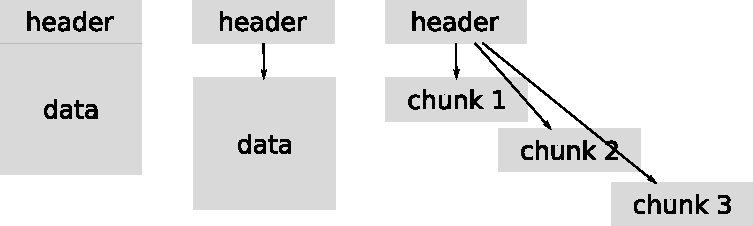
\includegraphics[width=\textwidth]{data_layout.pdf}
%caption{The three data layouts in \textit{DataSet}}
%\label{fig:datalayout}
%\end{figure}
\begin{figure}[ht!]
\resizebox{\textwidth}{!}{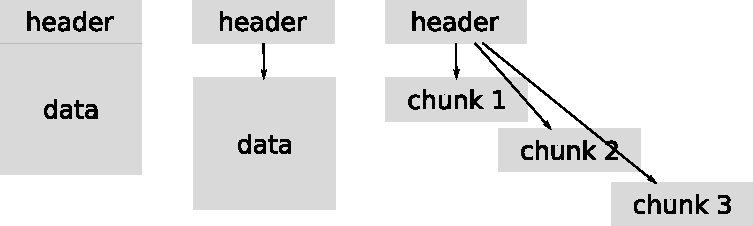
\includegraphics{data_layout.pdf}}
\caption{The three data layouts in \textit{DataSet}}
\label{fig:datalayout}
\end{figure}

If the data is sufficiently small \texttt{H5D\_COMPACT} will be used. In this layout the data address follows right after the header as shown on the left. When the data is bigger but still has a constant size \texttt{H5D\_CONTIGUOUS} is the right layout. This one allows that the address of the data can be arbitrary in memory and is saved in the header. The last layout \texttt{H5D\_CHUNKED} on the right is useful assuming the size of the data is unknown. The data will be divided continuously into chunks with constant size where the address will be saved in the header. This means when a chunk is full a new one gets allocated with its address saved into the header. As the perceptive reader can guess the last layout is of most relevance for this project. A simulation generates new data in each time step which in essence is ideal for the size of a chunk because it further allows to label each chunk to its corresponding time step. This will be later used to match data according to its time label.

\section{DataType}
\label{seq:datatype}
The language C++ itself supports data types such as int, double, char etc. but these cannot be used directly in a binary data format.
This is caused by different data representation which are not homogeneous across different operating systems and system architectures. For example the difference between little-endian and big-endian machines. Thus the library has its own definitions which are compatible across platforms which are incorporated into the different classes seen in figure \ref{graph:hierarchy}. It is intuitively clear from their names which classes must be used to describe which data types. For instance for writing floating point numbers the \textit{FloatType} class is used. In this object further changes of characteristics can be done such as changing from default IEEE representation. In this project the \textit{PredType} and \textit{CompType} are of most relevance. The \textit{PredType} is predetermined meaning there is no explicit constructor needed. From this class \textit{NATIVE\_INT} is used to write the respective time labels for the data. The \textit{CompType} class is utilized for writing complex numbers and also this class has to be explicit constructed which will be explained in section \ref{seq:datatypedec}.

\section{DataSpace}
\label{seq:dataspace}
To describe the dimensionality of our data the \textit{DataSpace} class is required. The construction of such a \textit{DataSpace} is straightforward. Firstly the library needs to know the number of dimensions of the desired space. Secondly it has know the number of elements in each dimension. For the second argument an array of \texttt{hsize\_t} is expected instead of \texttt{int} as described in section \ref{seq:internaltypes}. To give the reader an idea the following code depicts the \textit{DataSpace} of a time grid.

\begin{lstlisting}
int rank = 1;
hsize_t size[rank];
size[0]=number_of_timesteps;
DataSpace limited_timespace(rank,size);
\end{lstlisting}
The problem herein lies in the number of time steps which is known only at runtime but the constructor expects it at compiletime. This leads to another approach which is to define a unlimited \textit{DataSpace}. The library allows this if an additional optional argument is added. This argument has to be of the same data type as the second argument and contains the maximum size of each dimension. The library expects that this argument has to be greater or equal than the previous argument otherwise an exception is thrown. For an unlimited space a special state is used namely \texttt{H5S\_UNLIMITED}. The above example code changes to the following if an unlimited space is desired:
\begin{lstlisting}
int rank = 1;
hsize_t size[rank] = {1};
hsize_t maxsize[rank]={H5S_UNLIMITED};
DataSpace unlimited_timespace(rank,size,maxsize);
\end{lstlisting}

\section{PropList}
Most classes require a specific property list at the moment of construction which include additional information. Depending on the object a different property list is required. All these lists have a common base class namely \textit{PropList} as presented in figure \ref{graph:hierarchy}. The possibilities of these property lists excel the scope of this project easily therefore the default value is enough. The default values are shortly described in table \ref{table:default}.

\begin{figure}[ht!]
\centering
\begin{tabular}{|l|l|}
\hline
Default name value&Influence\\
\hline
\texttt{H5P\_FILE\_CREATE}&\textit{H5FILE} creation\\
\texttt{H5P\_FILE\_ACCESS}&\textit{H5FILE} access\\
\texttt{H5P\_DATASET\_CREATE}&\textit{DataSet} creation\\
\texttt{H5P\_DATASET\_XFER}&raw data transfer\\
\texttt{H5P\_MOUNT}&\textit{H5File} mounting\\
\texttt{H5P\_DEFAULT}&base value for all the above\\
\hline
\end{tabular}
\caption{Table of property list default values and their influence}
\label{table:default}
\end{figure}

Noteworthy for this project is only the \textit{DSetCreatePropList} mentioned in section \ref{seq:dataset} which will be explained in the next section \ref{seq:dscpl}.

\subsection{DSetCreatePropList}
\label{seq:dscpl}
From section \ref{seq:dataset} a \textit{DSetCreatePropList} object is demanded for creating a \textit{DataSet}. As the perceptive reader can guess this property list is used to determine the data layout shown in figure \ref{fig:datalayout}. The property list is responsible for setting the layout to \texttt{H5D\_COMPACT}. This is important because only data with this layout can be dynamically extended later on during a simulation. 

\section{Attribute}
Additionally to writing data in binary format it should also incorporate saving corresponding meta data. This can be easily done with \textit{Attributes} which must be attached to an affiliated \textit{Group} or \textit{DataSet}. The allocation of such an \textit{Attribute} is similar to a \textit{DataSet} meaning a \textit{DataType} and \textit{DataSpace} is also demanded. For its property list only the \texttt{H5P\_DEFAULT} is allowed which the library enforces otherwise an exception is thrown.

\chapter{Writer Template}
\section{Link to Eigen library}
As mentioned in background \ref{seq:background} the simulation boils down to propagating the set \{q,p,Q,P,S\} where q and p are $D$ dimensional real-valued vectors, Q and P complex $DxD$ matrices and S the global complex phase. A possible interface to manage these matrices and vectors is the Eigen library. The definition of an Eigen matrix has the following form:
\begin{lstlisting}
Eigen::Matrix<std::complex<double>,row_dim,column_dim> mat;
\end{lstlisting}
Note that this is a class template over three parameters namely type, row-dimension and column-dimension. Therefore the overall implementation will also be a template. In the current version only scalar \textit{Hagedorn} wavepackets are supported thus only one dimension parameter $D$ is utilized but the framework can still easily be extended in further works. As discussed in section \ref{seq:datatype} normal types are not writable hence the type is defined through the library. This declared type is not necessarily the same as the template argument from Eigen but is still similar enough to permit basic transformation functions.

\section{DataType Declaration}
\label{seq:datatypedec}
In this context simulation means manipulating complex numbers. To build a \textit{DataType} the library needs access to its members thus the standard \texttt{complex} class cannot be utilized. Therefore a \texttt{struct} is most suitable for defining the fundamental structure since all its members are by default public accessible. Hence the declaration of complex numbers looks like this:
\begin{lstlisting}
struct ctype
{
  double real;
  double imag;
} instance_of_ctype;
\end{lstlisting}
This can now be used by the library to create the corresponding \textit{DataType} which in this case the \textit{CompType} is most suitable because \texttt{ctype} is a composition of simple data types. To be compatible with python the same labels for its members has to be used which result in the following code:
\begin{lstlisting}
CompType nctp_(sizeof(instance_of_ctype));
nctp_.insertMember("r",HOFFSET(ctype,real), PredType::NATIVE_DOUBLE);
nctp_.insertMember("i",HOFFSET(ctype,imag), PredType::NATIVE_DOUBLE);
\end{lstlisting}
Worth noting is that the constructor of \textit{CompType} relies on the \texttt{sizeof} operator which tells how many bytes for an instance of this type is needed. The string labels "r" and "i" are utilized for the real respective the imaginary part of a complex number. \texttt{HOFFSET} is a simple function which returns at which position counted in bytes the second argument is located in the first argument. In this simple case because one double is saved in $8$ Bytes \texttt{real} is at position "0" and \texttt{imag} is at position "8". Finally the last argument is the type inserted at this position. Since already discussed in section \ref{seq:datatype} \texttt{double} cannot be used directly but the library provides these definitions through the \textit{PredType} class. The members of \textit{PredType} are constant and are fixed through the C++ language itself.\\

\section{Constructor}
Since the data type declaration has only to be initialized once it is suitable to pack it into the constructor of this writer template. The constructor only expects one string argument namely the filename. Therefore the the constructor can be written accordingly:
\begin{lstlisting}
template<int D>
...
//ctor
hdf5writer(std::string name):filename_(name), nctp_(sizeof(instanceof)),file_(filename_,H5F_ACC_TRUNC)
{
	nctp_.insertMember("r",HOFFSET(ctype,real), PredType::NATIVE_DOUBLE);
	nctp_.insertMember("i",HOFFSET(ctype,imag), PredType::NATIVE_DOUBLE);
}
\end{lstlisting}
Observe that there are two implicit constructor calls after instantiation of the filename. For the former refer to section \ref{seq:datatypedec} for the latter to section \ref{seq:h5file}.

\section{Write options}
To enable customization about what and when something is written an additional layer was inserted. This was done with functions which set the desired configuration. In the current implementation there are three choices to make. By default writing \textit{Hagedorn} wavepackets is enabled and writing norm and energies are disabled with a boolean. As already mentioned in section \ref{seq:dataset} for each chunk written also a time label is attached. This was achieved by writing for each important \textit{DataSet} an additional \textit{DataSet} at the same level with the same length where each entry is an \texttt{int} symbolizing the number of time steps passed since the beginning of the simulation. These are shown in figure \ref{graph:file} where "timegrid" was used in its name. The corresponding customization thereof is to set the difference between two consecutive entries. More precisely it is the choice if a \textit{DataSet} should be written in each time step($d=1$) or every second time step($d=2$) etc. The supported functions are listed subsequently:
\begin{lstlisting}
set_write_packet(true|false);
set_write_norm(true|false);
set_write_energies(true|false);
set_timestep_packet(1|2|3|...);
set_timestep_norm(1|2|3|...);
set_timestep_energies(1|2|3|...);
set_timestep_ekin(1|2|3|...);
set_timestep_epot(1|2|3|...);
\end{lstlisting}

\section{DataSet paths}
The structure in figure \ref{graph:file} is fixed in the implementation as it is analogous to the python generated data. Furthermore the names of all \textit{Groups} and \textit{DataSets} are also already determined. The data test is build on these as well. This can be problematic once a change happens in the python or C++ implementation where the structure is affected. Luckily the library throws an invalid path exception if such a change occurs where the paths are no longer valid. Future work could include to make data test path independent for \textit{DataSets}.

\section{Prestructure}
\label{seq:prestructure}
This function is a bundle of steps which either have to be done prior or are constant during the writing process. The function definition is shown subsequently:
\begin{lstlisting}
template<class MultiIndex>
prestructuring(ScalarHaWp<D,MultiIndex> packet,double dt);
\end{lstlisting}
The dimension $D$ and the class \texttt{MultiIndex} are prerequisite for constructing a scalar \textit{Hagedorn} wavepacket and is detailed explained in the thesis of Michaja B\"osch \cite{bt_michajab}. A scalar \textit{Hagedorn} wavepacket includes a matrix of coefficients and the set \{q,p,Q,P,S\}. The coefficient dimension is dependent on $D$ and \texttt{MultiIndex} therefore the number of coefficients is calculated and stored first in this function. Next the \textit{Groups} of figure \ref{graph:file} is set. Additionally some \textit{Attributes} are attached to the root group such as the time step $dt$. As discussed in section \ref{seq:dataset} each \textit{DataSet} has to be chunked according to a time step. Hence this chunk dimension is set in the next step for all \textit{DataSets} specified in the write options. E.g. for a packet the chunk-dimension for the coefficients, q, p, Q, P, and S have to be set into a instance of \textit{DSetCreatPropList} individually. 
For instance a chunk-dimension is declared in the following form:
\begin{lstlisting}
hsize_t chunk[3] = {1,2,2};//{time_dim,row_dim,column_dim}
\end{lstlisting}
Before it is possible to allocate all \textit{DataSets} according to figure \ref{graph:file} also individual \textit{DataSpaces} have to be declared. Luckily it is possible to reuse all chunk-arrays as arguments for their own \textit{DataSpace} with the additional array argument according to section \ref{seq:dataspace}. Now all building blocks are ready to allocate in the next step all \textit{DataSets}. It can be observed that there is a source and destination \textit{DataSpace} with a selection in each time step. The \textit{DataSpace} is the space of possible positions where data can be written to whereas the a hyperslab is used for the actual selection within the space. The destination \textit{DataSpace} grows over time within the file and thus is not constant. Different from the destination, the source \textit{DataSpace} and its selection is constant and therefore can be fixed in this step for the whole simulation. The workings of a hyperslab as selection is explained in the next section \ref{seq:selection}.

\section{Selection}
\label{seq:selection}
As already mentioned in the previous section \ref{seq:prestructure} a selection within a \textit{DataSpace} is represented with a hyperslab. A hyperslab consists of four arrays namely:
\begin{lstlisting}
hsize_t start[3] = {time_label,1,1};
hsize_t count[3] = {time_label,3,2};
hsize_t block[3] = {time_label,1,1};
hsize_t stride[3] = {time_label,2,2};
\end{lstlisting}
Notice that the first dimension is always reserved for the time dimension. The implementation has an internal index for storing the current simulation step which is used as the label. Thus only the index for the next time step has to be incremented without altering the code for the selection. The following figure \ref{fig:hyperslab} illustrates why four arrays are required to represent a hyperslab.

\begin{figure}[ht!]
\centering
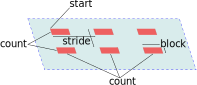
\includegraphics[scale=1.8]{selection.pdf}
\caption{hyper-slab illustration}
\label{fig:hyperslab}
\end{figure}
%TODO explaining figure

The selection is done by the \textit{DataSpace} itself whereas the \texttt{H5S\_SELECT\_SET} argument is recommended to overwrite the old selection.
\begin{lstlisting}
dataspacename.selectHyperslab(H5S_SELECT_SET, count, start, stride, block);
\end{lstlisting}
In case that a continuous block of data is written the last two arguments can be omitted.
\begin{lstlisting}
dataspacename.selectHyperslab(H5S_SELECT_SET, count, start);
\end{lstlisting}


\section{Transformation}
As previously discussed to write data we use our own created data type \textit{nctp}. To write a buffer we need now a pointer of \texttt{ctype}. As such our transformation functions take an \texttt{Eigen::Matrix} with arbitrary template arguments and copies the raw data into a \texttt{std::vector<ctype>} reference. An important implementation detail for data management is the usage of \texttt{std::vector} because the operation system assumes the allocation and deallocation of \texttt{std} objects. Thus our code is much safer in respect to data leaks and data corruption. The \textit{Eigen} library self-manages its matrix objects. To extract \texttt{ctype} pointer from the \texttt{std::vector} object is simple by using the \texttt{.data()} function call.

\section{Writing} 
The writing function call from the HDF library has the following form:
\begin{lstlisting}
datasetname.write(void* src,DataType type,DataSpace srcspace,DataSpace dstspace);
\end{lstlisting}
We already have all tools available to use this function. The \texttt{src} is delivered from the transformation section, \texttt{type} from the declaration section and \texttt{srcspace}, \texttt{dstspace} from the prestucturing sectoin or selection section respectively.

\section{Extension}
For extending a \textit{DataSet} we need the new dimension in a \texttt{hsize\_t} array which is used as the extension. Note here that only chunked \textit{DataSets} are possible to extend with the following call:
\begin{lstlisting}
datasetname.extend(hsize_t extension);
\end{lstlisting}
Also note this function call can also be used to reduce the dimension if the used array \texttt{extension} is smaller then the existing \textit{DataSet}. To know the current position of the data an \texttt{int index} is used for every existing \textit{DataSet}. This index is also used in setting the dimension of the \texttt{hsize\_t extension} array.

\section{Update}
After the extension of a \textit{DataSet} the library doesn't automatically also update the corresponding \textit{DataSpace} which was used in the selection section. As such this is done in this update section. Also the corresponding \texttt{index} to the \textit{DataSet} is incremented in this step. The library provides an easy way to use the extended \textit{DataSet} to set the new \textit{DataSpace} namely:
\begin{lstlisting}
dataspacename = datasetname.getSpace();
\end{lstlisting}
which is done for every existing \textit{DataSet} in the file.
\section{Poststructure}
After the last time step of the simulation we have to finalize our \textit{DataSet} and structures used. This is done in this section. From our implementation we know that also in the last time step we did extend the \textit{DataSet}. As such the last extension will be reversed. Afterwards every structure from the library has to be freed from memory. The system does this automatically for all structures allocated on the stack. For structures which are on the heap because they were allocated with the \texttt{new} operator we have to free them ourselves. This step can be cumbersome because mostly we don't know anymore which object has internally somewhere a reference to it and therefore it is unsafe data management. The implementation avoids this problem by using the \texttt{new} operator to allocate \texttt{std::shared\_ptr} objects which will be managed by the standard library the same as the \texttt{std::vector}. As such the data management is primarily done by the system and not by the implementation.
\section{Inner workings in a picture}
The following figure \ref{fig:illustration} shows the lifetime of a \textit{DataSet} in this implementation. The start signalizes the use of the constructor to allocate the object.
\begin{figure}[ht!]
\resizebox{\textwidth}{!}{
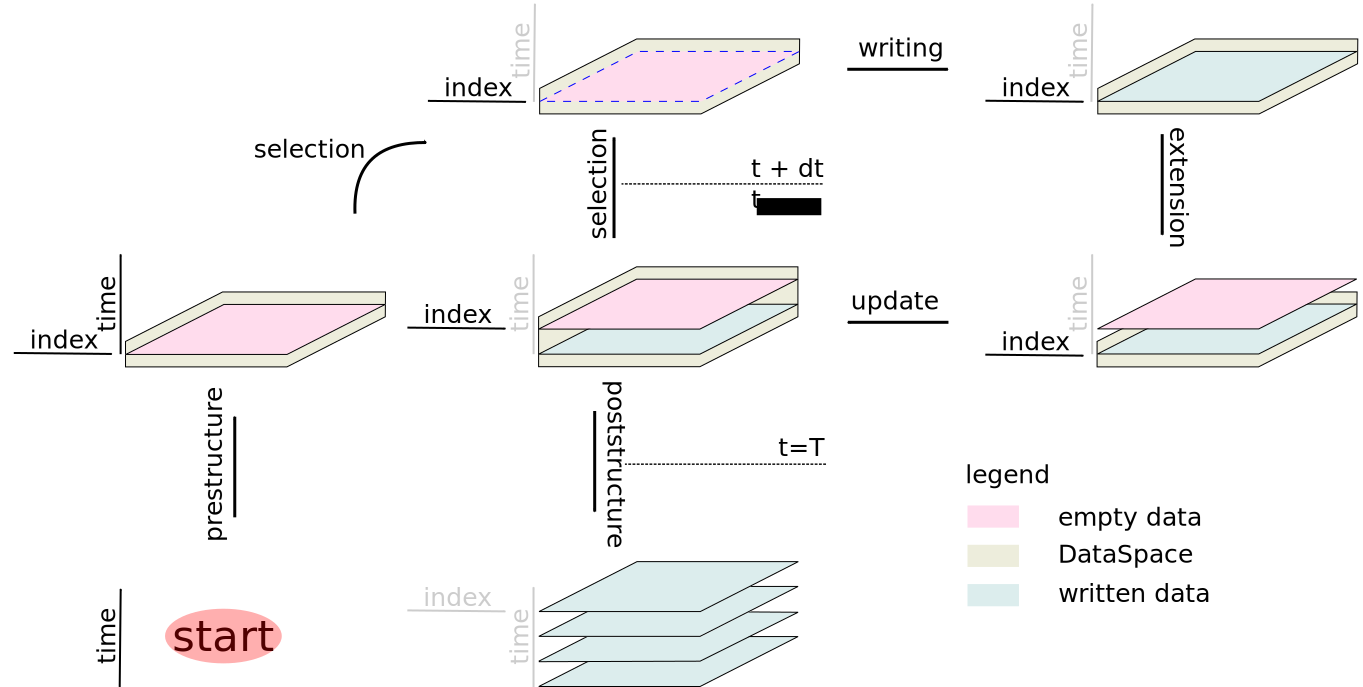
\includegraphics[scale=1.0]{writing_dataset.pdf}
}
\caption{Illustration of inner workings for a \textit{DataSet} in the simulation}
\label{fig:illustration}
\end{figure}

\section{Usage in a simulation main file}
Note that this implementation is only able to write scalar \textit{Hagedorn} wave packets with the normal \textit{Hagedorn} parameter set for the moment. Further work includes to either extend this HDF5 writer template with matching functions for more complicated \textit{Hagedorn} wave packets or to generalize the template on these packets. In the simulation the packet and its parameter set is constructed in the following form:
\begin{lstlisting}
...
wavepackets::HaWpParamSet<D> param_set(q,p,Q,P,S);
...
wavepackets::ScalarHaWp<D,MultiIndex> packet;
...
\end{lstlisting}
%
%TODO reference zu Michja wie ScalarHawp implementiert isch
%
Hence our HDF5 writer template is constructed and used in the following way:
\begin{lstlisting}
... //setting simulation variables, options etc.

//constructor of this template implementation
io::hdf5writer<D> writer("simulation_filename.hdf5");

//optional setup write options
bool write_packet,write_energy,write_norm;
write_packet=true;//default value
write_energy=false;//default value
write_norm=false;//default value
writer.set_write_energy(write_packet);
writer.set_write_norm(write_energy);
writer.set_write_packet(write_norm);
int packet_stepsize,energy_stepsize,norm_stepsize;
packet_stepsize=1;//default value writing every time step
energy_stepsize=1;//default value writing every time step
norm_stepsize=1;//default value writing every time step
writer.set_timestep_packet(packet_stepsize)
writer.set_timestep_energy(energy_stepsize)
writer.set_timestep_norm(norm_stepsize)

//optional setup write paths
std::string datablockstring,wavepacktstring,packetgroupstring;
std::string coefficientgroupstring,energiesgroupstring;
std::string normsgroupstring,observablesgroupstring;
//default paths see figure @\ref{graph:file}@
datablockstring="/datablock_0";
wavepacktstring="/wavepacket";
packetgroupstring="/Pi";
coefficientgroupstring="/coefficients"
energiesgroupstring="/energies"
normsgroupstring="/norm";
observablesgroupstring="/observables";
writer.set_datablockstring(datablockstring);
writer.set_wavepacketstring(wavepacktstring);
writer.set_packetgroupstring(packetgroupstring);
writer.set_coefficientgroupstring(coefficientgroupstring);
writer.set_energiesgroupstring(energiesgroupstring);
writer.set_normsgroupstring(normsgroupstring);
writer.set_observablesgroupstring(observablesgroupstring);

//prestructuring step
writer.prestructuring<MultiIndex>(packet,dt);

//simulation loop body
for(real_t t = 0; t < T; t += dt)
{
	real_t ekin=observables::kinetic_energy<D,MultiIndex>(packet);
	real_t epot=observables::potential_energy<ScalarMatrixPotential<D>,D,MultiIndex,TQR>(packet,V);
	writer.store_packet(packet); //function call for storing packet in file
	writer.store_energies(epot,ekin); //function call for storing energies in file
	writer.store_norm(packet); //function call for storing norm in file	
}

//finalization with postructure
writer.poststructuring();
\end{lstlisting}
Remember that only the constructor, prestructuring and poststructuring are always mandatory independent of the simulation. Also note that if write option of norm and/or energies is set to true but the \texttt{.store\_...} function call is missing that an error message will be printed without aborting the simulation. 

\chapter{Data Test}

\section{Introduction to GoogleTest}
There are two main ways to test objects with this framework. For the interested reader a more detailed documentation can be found in the git repository \cite{googletestdoc} where the Primer.md and AdvancedGuide.md examples are strongly suggested. Of importance is to define a test class for reusing certain objects for all tests. These objects in this case are the two \textit{H5Files}, the \textit{DataType} used in the writing process and the \textit{Attributes} saved in the root group of the two files. One of these \textit{Attributes} is the used time step $\Delta t$ in the simulation which will be needed later for a data matching.

\section{The Main C++ File}
The data test main file is of the following structure:
\begin{lstlisting}
#include "gtest/gtest.h"
int global_argc;
char** global_argv;
...

class TestHDF : public ::testing::Test
{
	protected:
	TestHDF();
	virtual ~TestHDF();
	void SetUp();
	void TearDown();
	void time_matching(...);
	
	struct ctype{...};
	H5File cppfile;
	H5File pyfile;
	CompType nctp;
	double dt_cpp;
	double dt_py;
	...
};

TEST_F(TestHDF,Testpacket)
{...}
TEST_F(TestHDF,Testenergies)
{...}
TEST_F(TestHDF,Testnorm)
{...}

int main(int argc,char* argv[])
{
	global_argc=argc;
	global_argv=argv;
	::testing::InitGoogleTest(&argc,argv);
	return RUN_ALL_TESTS();
}
\end{lstlisting}

%TODO overwork
Note that \texttt{TEST\_F} are test fissures which uses the same class object \texttt{TestHDF}. In the constructor the filenames are loaded in the \texttt{H5File} objects and the \textit{CompType} is also set the same as in section \textit{DataType} declaration. For each test fissure the \texttt{SetUp} function is used for further construction and at the end cleaned with \texttt{TearDown} function. To transfer the filenames, which are delivered over the command line arguments, global variables are used. In the respective test fissures the data of the two files will be compared relative to an absolute tolerance error. Hereby it has to be known which time points can be compared to in a general case. This is done with the \texttt{time\_matching} function which saves the matching time points in vector, where every entry are two indices, and as arguments two paths, represented as strings with the same form as in group section, to the respective time grid \textit{DataSet}.

\chapter{Conclusion}

